%!TEX root = ../../Compte-rendu.tex
\subsection{Résultats}

\begin{figure}[H]
	\begin{center}
		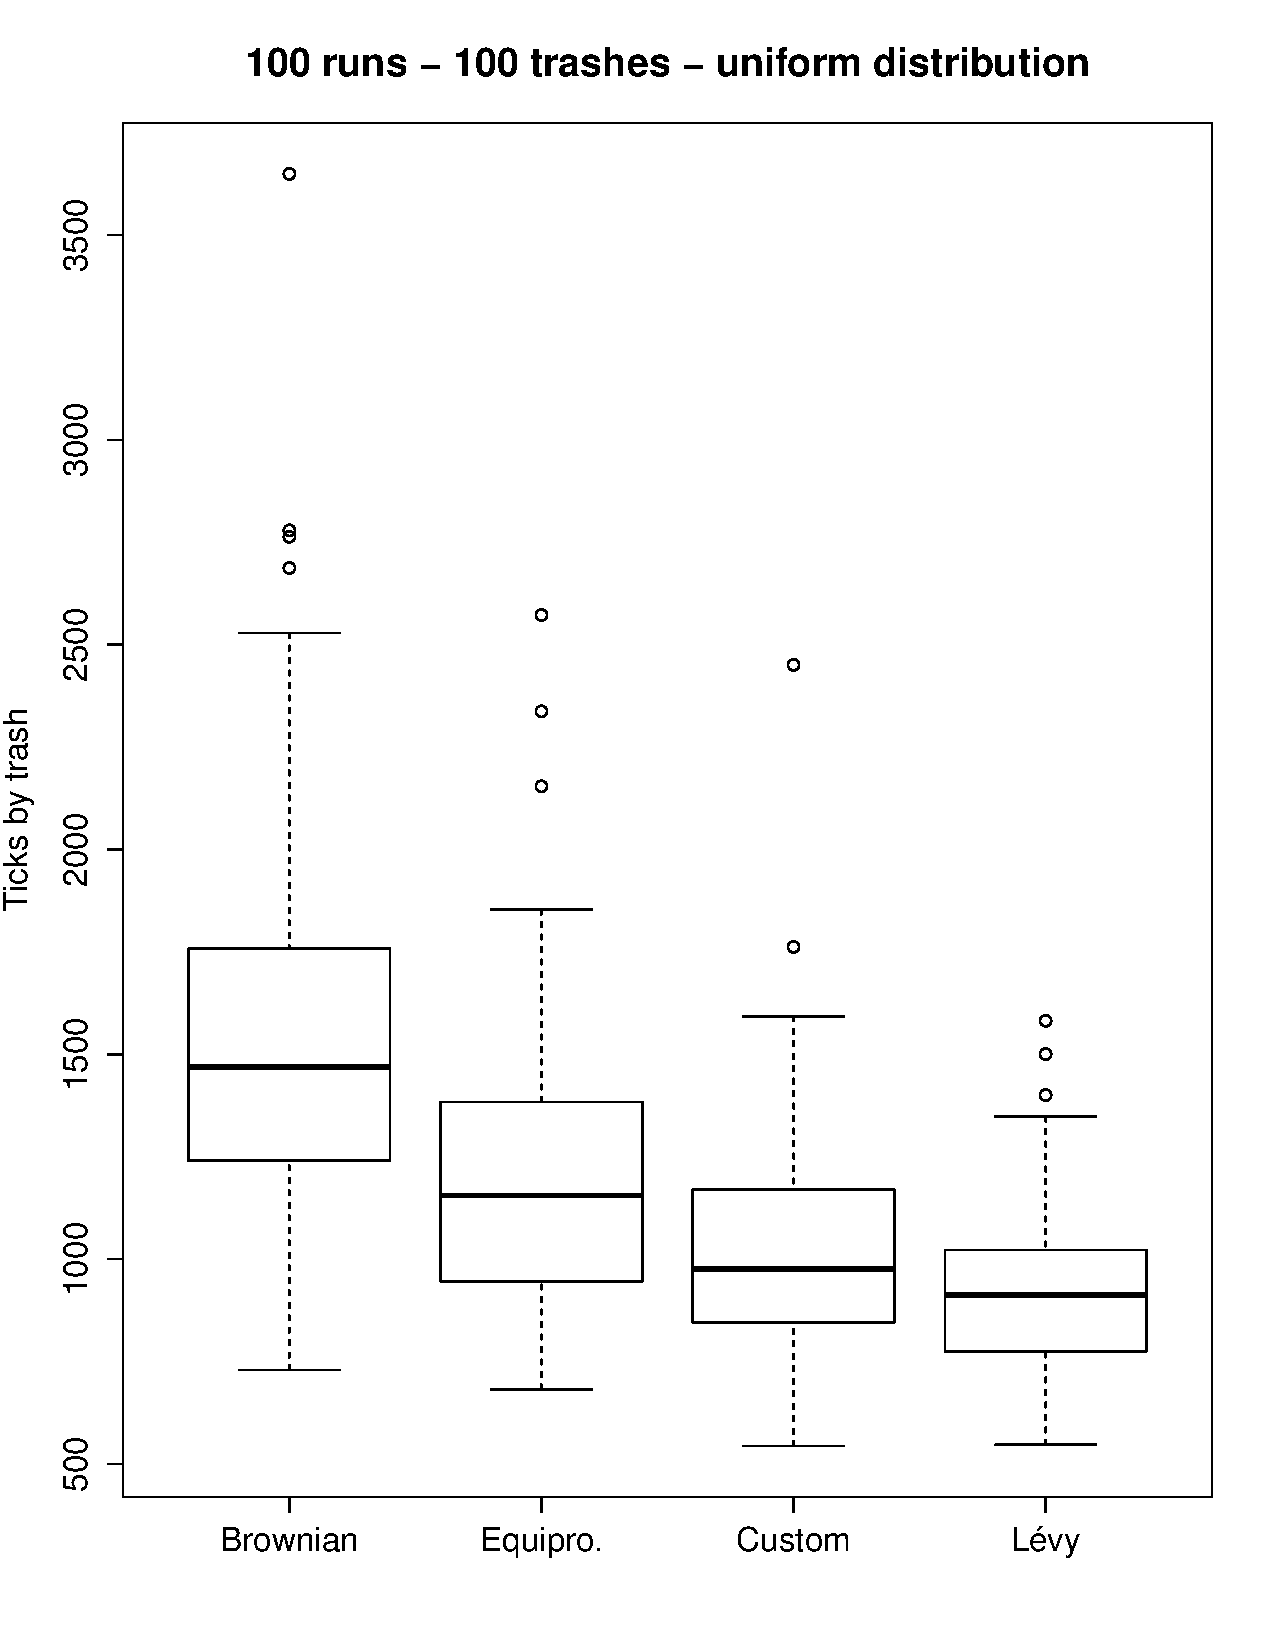
\includegraphics[height=8cm]{diagrams/100TrRnd_all.pdf}
		\caption{}
		\label{fig:100Trashes_Rnd}
	\end{center}
\end{figure}

Nous avons pour les différentes stratégies les médianes suivantes :

\begin{tabular}{ | c | c | }
	\hline
	\multicolumn{2}{ | c | }{Médianes pour la 100 débris distribués uniformément} \\
	\hline
	Brownian & 1468.673 \\
	Equiprobable & 1155.213 \\
	Custom & 974.9208 \\
	Lévy & 911.797 \\
	\hline
\end{tabular}
